\documentclass[a4paper,10pt,twocolumn,uplatex]{jsarticle}
\usepackage{style/nislab}

%---------------------------------------------------------------------
% レジュメ種別・日付設定(要変更)
% \type{} 1:修士論文諮問会 2:卒業論文発表会 else:月例発表会
\type{3}
\year{2021}
\month{7}
\date{10}

%---------------------------------------------------------------------
% ページ番号設定(要変更)
\setcounter{page}{9}

%---------------------------------------------------------------------
\begin{document}
%---------------------------------------------------------------------
% タイトル作成部分(要変更)
% \maketitle{タイトル}{title}{名前}{name}
\maketitle{スマートホームにおけるSDNを用いたトラフィック監視による不正アクセス防御手法の検討}
{A Study on Unauthorized Access Protection Method by Traffic Monitoring Using SDN in Smart Home}
{塚﨑 拓真}
{Takuma Tsukasaki}

%---------------------------------------------------------------------
\section{はじめに}
近年,IoT(Internet of Things)が注目を集めるようになり,今後あらゆるものがネットワークに接続され,利用されることが予想される.
現在,IoT機器が様々なところに置かれるようになり,以前のパソコンやスマートフォンに限らず,現在ではテレビやゲーム機,Webカメラ,冷蔵庫などの家電などがインターネットに繋がり,情報を通信するようになっている.
それに伴い,ネットワークないには様々な端末や機器が混在することになる.ホームネットワークは情報家電などの普及も加わり,その形態が多様化していくと考えられる.\par
しかし,IoTの登場で利便性が高まる一方で,これまでのネットワークに接続されていないモノが接続されることにより,セキュリティ上のリスクが高まっている\cite{guideline}.
IoTはセキュリティを考慮せずに開発されたものが多く,悪意のある攻撃者によるサイバー攻撃の標的になりやすく,特に不正アクセスが多発している.
これらが各種端末やネットワークごとに顕在した場合,個別に対処するとコストや時間がかかってしまうため,脅威に対し一括に対処する必要がある.
ホームネットワーク内には異なる規格のハードウェアやそれらに搭載される様々なアプリケーションが混在しているため,それら全てに対応したシステムの構築や更新を続けるのは困難である.
ホームネットワーク内には異なる規格のハードウェアやそれに対応したソフトウェアとして構築するのではなく,ホームネットワーク内で通信するのであれば,どの端末も必ず利用するネットワークを利用したシステムを構築することが望ましい.

%---------------------------------------------------------------------
\section{関連研究}
村上らは,OpenFlowを用いてホームネットワーク内に,動的な認証システムを構築し,不正アクセスによる被害を軽減する手法を提案した\cite{related}.
本提案方式では,認証時に頻繁に利用される情報を用いることで,ネットワークに接続する端末を制限すると共に,万が一認証が突破された場合でも不正アクセスが検出できるシステムを構築した.
しかし,1度入られてしまったら,攻撃されてしまう.
現在のスマートホームデバイスは,クラウド上のシステムと連携することで,デバイス間の連携を可能にしているが,今後はホームネットワーク内で閉じたデバイス間の通信によって連携を行う形になることが想定される\cite{d2d}.
また,同じホームネットワークに他の多くの機器が何の制限もなく接続されているという事実を利用して,マルウェアをインストールする.
カメラに搭載されたマルウェアは,ローカルネットワーク上で他の潜在的に脆弱なデバイスをスキャンし,例えばよく知られたセキュリティ上の欠陥を利用してそれらのデバイスにアクセスし,同じまたは異なるマルウェアのコピーをさらにインストールしようとする.
感染した機器がマルウェアの支配下に置かれると,個人情報の漏洩など,スマートホームネットワーク自体に被害を及ぼすだけでなく,DDoS攻撃への加担やサービスの操作など,他の悪意ある活動を行う可能性がある\cite{disap}.

%---------------------------------------------------------------------
\begin{figure}[!tb]
  \centering
  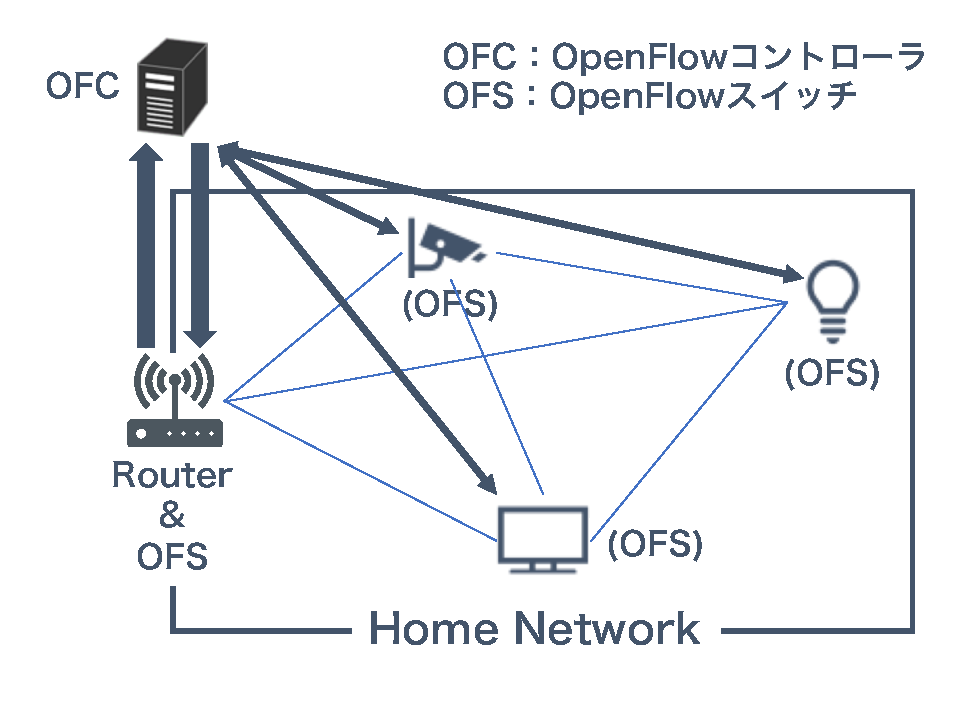
\includegraphics[width=\linewidth]{img/architecture.eps}
  \caption{提案手法のアーキテクチャ}
  \label{fig:architecture}
\end{figure}

%---------------------------------------------------------------------
\section{提案手法}
前述の問題点を受けて,関連研究は、万が一認証が突破された場合でも、不正アクセスが検出できるとしていた。しかし、デバイス間通信が想定され、感染拡大を防ぐことを考慮し、ホームネットワーク内においての検知も必要である。
OpenFlowを利用することで、ホームネットワークに適した形で、不正な通信の検知を実現する。
OpenFlowを利用することで、既存IoT機器や異なる規格などに対応できる。また、動的に接続を管理することで、不正通信による被害を軽減する。

\subsection{想定環境}
閉ざされたホームネットワークにおいて、デバイス間の通信、ルーター・デバイス間の通信を想定する。
また、デバイス数は一般的に利用されているルーターの推奨接続台数である10\textasciitilde15台を想定する。

\subsection{概要}
OpenFlowを用いて、トラフィック監視を行うことで、ホームネットワーク内で行われる通信を制限する。
既存IoT機器にOpenFlowスイッチの機能を導入することは困難であると考え、OpenFlowスイッチの機能を持った仮想デバイスを既存IoT機器の前に用意する。
通信が行われる際に、仮想デバイスを通して、OpenFlowコントローラに接続し、トラフィック情報から通信の許可を判断する。

\subsection{動作手順}
本提案手法の動作手順を以下に述べる.

\begin{enumerate}
  \item 接続要求機器は仮想デバイス(OFS)に通信する
  \item 仮想デバイス(OFS)はOpenFlowコントローラに対して、Packet Inメッセージを送信
  \item OpenFlowコントローラはトラフィック情報を調査
  \item 正当な通信の場合、OpenFlowコントローラは送信元機器に対して、許可メッセージとして、Flow Modメッセージを送信
  \item 不正な通信の場合、OpenFlowコントローラは送信元機器に対して、不許可メッセージとして、Flow Modメッセージを送信
  \item OpenFlowコントローラは送信元機器に対して、Packet Outメッセージを送信
\end{enumerate}

\subsection{トラフィック情報}
本提案手法で通信の許可を判断するトラフィック情報として、以下の3点を用いる。

\begin{itemize}
  \item パケットヘッダー
  \item パケットの長さ
  \item 周期性
\end{itemize}

%---------------------------------------------------------------------
\section{評価}

%---------------------------------------------------------------------
\section{まとめ・今後の課題}

%---------------------------------------------------------------------
% Bibliography
\footnotesize{
  \begin{thebibliography}{99}
    \bibitem{guideline} IoT推進コンソーシアム, 総務省, 経済産業省, "IoTセキュリティガイドライン ver 1.0", 2016.
    \bibitem{related} 村上萌, 中村嘉隆, 高橋修, "OpenFlowを用いたホームネットワークへの接続端末制御による不正アクセス防御手法の提案", 研究報告コンピュータセキュリティ(CSEC), Vol.2016-CSEC-72, No.29, pp.1-6, 2016/2.
    \bibitem{d2d} C. Vallati, A. Virdis, E. Mingozzi and G. Stea, "Mobile-Edge Computing Come Home Connecting things in future smart homes using LTE device-to-device communications", IEEE Consumer Electronics Magazine, Vol.5, No.4, pp. 77-83, 2016.
    \bibitem{disap} M. Serror, M. Henze, S. Hack, M. Schuba, and K. Wehrle, "Towards In-Network Security for Smart Homes", Proceedings of the 13th International Conference on Availability, Reliability and Security (ARES 2018), No.18, pp.1–8, 2018.
  \end{thebibliography}
}

%---------------------------------------------------------------------
\end{document}
%---------------------------------------------------------------------
